\documentclass[journal]{IEEEtran}

% ─── Packages ────────────────────────────────────────────────────────────────
\usepackage{amsmath,amssymb,amsthm}
\usepackage{graphicx}
\usepackage{booktabs}
\usepackage{multirow}
\usepackage{hyperref}
\usepackage{cite}
\usepackage{algorithm}
\usepackage{algpseudocode}
\usepackage{xcolor}
\usepackage{subcaption}
\usepackage{array}
\usepackage{url}

% ─── Theorem environments ────────────────────────────────────────────────────
\newtheorem{theorem}{Theorem}
\newtheorem{definition}{Definition}
\newtheorem{proposition}{Proposition}
\newtheorem{remark}{Remark}

% ─── Custom commands ─────────────────────────────────────────────────────────
\newcommand{\R}{\mathbb{R}}
\newcommand{\SSR}{\mathcal{S}}
\newcommand{\Loss}{\mathcal{L}}
\newcommand{\Net}{\mathcal{N}}
\newcommand{\bx}{\mathbf{x}}
\newcommand{\by}{\mathbf{y}}
\newcommand{\bz}{\mathbf{z}}
\newcommand{\bV}{\mathbf{V}}
\newcommand{\btheta}{\boldsymbol{\theta}}
\newcommand{\blambda}{\boldsymbol{\lambda}}
\newcommand{\relu}{\mathrm{ReLU}}

% ─── Title and authors ───────────────────────────────────────────────────────
\title{Deep Learning-Based Characterization of Power System Static Security Regions Using Multi-Solution OPF Test Cases}

\author{
  \IEEEauthorblockN{[Authors]}\\
  \IEEEauthorblockA{[Institution]}
  \thanks{Manuscript received ---; revised ---.
  Corresponding author: [email].
  Code available at: \url{https://github.com/yourusername/PowerSSR-DL}}
}

\begin{document}

\maketitle

% ─────────────────────────────────────────────────────────────────────────────
\begin{abstract}
% ─────────────────────────────────────────────────────────────────────────────
Characterizing the static security region (SSR) of power systems — the set of
all load operating points for which a feasible AC power flow solution satisfying
all operational constraints exists — is a fundamental problem for real-time
security assessment. Classical approaches rely on iterative power flow solvers,
which are computationally prohibitive for large-scale systems or online
applications. This paper proposes \textbf{SSR-DL}, a deep learning framework
that directly learns the SSR boundary from data, enabling near-instantaneous
security classification at inference time.

Our approach features three innovations: (i)~a dual-branch neural architecture
with a shared feature extractor and separate classification and physics heads;
(ii)~Lagrange dual training with learnable multipliers for soft enforcement of
voltage and line-flow constraints; and (iii)~a contrastive boundary loss that
sharpens the predicted decision boundary near the true SSR frontier. We
evaluate SSR-DL on the publicly available multi-solution OPF benchmark cases
from Bukhsh et al.\ (2013) — specifically WB2, WB5, and the modified IEEE
9-bus system (case9mod) — which are specifically designed to exhibit multiple
local OPF solutions, making security region characterization particularly
challenging. SSR-DL achieves \textbf{F1 = 1.000} on the WB2 case (feasibility
rate 2.5\%) and \textbf{F1 = 0.997} on case9mod, consistently outperforming
baseline feedforward and physics-informed neural networks. The full code and
trained models are released as open source.
\end{abstract}

\begin{IEEEkeywords}
Static security region, feasibility region, optimal power flow, deep learning,
physics-informed neural network, Lagrange dual method, power system security
assessment.
\end{IEEEkeywords}

% ─────────────────────────────────────────────────────────────────────────────
\section{Introduction}
\label{sec:intro}
% ─────────────────────────────────────────────────────────────────────────────

Power system security assessment requires determining, in near real time,
whether a given operating point will remain within acceptable limits under
normal and contingency conditions. The \emph{static security region} (SSR)
formalizes this as a set in the space of controllable variables (load demands,
generation dispatch) within which all AC power flow constraints — voltage
magnitudes, branch flow limits, reactive power limits — are simultaneously
satisfied~\cite{jiang2017feasibility}.

Traditional SSR computation relies on iterative AC power flow or optimal power
flow (OPF) solvers. Although mature and accurate, these methods scale poorly:
a single AC-OPF solve for a 300-bus system may take seconds on a workstation,
while real-time applications demand sub-millisecond responses across thousands
of candidate operating conditions. Data-driven and machine-learning approaches
have emerged as a promising avenue to reduce this computational burden by
amortizing expensive offline computation into fast online inference
\cite{donti2021machine,pan2023deepopf}.

\subsection{Related Work}

\textbf{OPF surrogate models.} A substantial body of work trains neural
networks to \emph{predict} optimal dispatch decisions given load inputs
\cite{pan2023deepopf,chen2022learning}. These models are fast at inference but
produce \emph{point predictions} of the optimal solution rather than
characterizing the feasibility boundary.

\textbf{Feasibility-seeking methods.} Nguyen and Donti~\cite{nguyen2025fsnet}
propose FSNet, which appends a differentiable feasibility-seeking correction
step to a standard NN predictor, guaranteeing constraint satisfaction.
Liang et al.~\cite{liang2023homeomorphic} learn a homeomorphic mapping from the
unit ball to the constraint set, enabling strict feasibility via projection.
Kim and Kim~\cite{kim2025deeplagrange} embed power flow equations as hard
constraints via implicit differentiation and enforce inequalities through
Lagrange dual training.

\textbf{Security region characterization.} Jiang and Chiang~\cite{jiang2017feasibility}
develop a dynamical-systems approach that analytically characterizes OPF
feasibility regions as stable equilibrium manifolds of a quotient gradient
system, revealing their potentially disconnected topology. Fan et
al.~\cite{fan2024error} quantify the Hausdorff distance between convex
approximation feasibility regions and the true nonconvex AC-OPF feasibility
region. However, neither approach learns a fast, generalizable model of the
security boundary.

\textbf{Multi-solution OPF.} Bukhsh et al.~\cite{bukhsh2013local} identify
test cases for which the AC-OPF problem admits multiple locally optimal
solutions, highlighting the nonconvexity of the feasibility region. These
cases provide particularly challenging benchmarks for security region methods
because the SSR may be small, irregular, or have non-trivial topology.

\subsection{Contributions}

This paper makes the following contributions:

\begin{enumerate}
  \item We formulate SSR characterization as a binary classification problem
    in the load demand space, and propose SSR-DL, a neural network architecture
    incorporating (a)~dual-branch design with physics head, (b)~Lagrange dual
    training with learnable constraint multipliers, and (c)~contrastive
    boundary loss.

  \item We provide \emph{complete Python implementations} of the Bukhsh et
    al.~(2013) multi-solution OPF test cases in pandapower, enabling
    reproducible experimentation without MATPOWER.

  \item We conduct systematic experiments on WB2, WB5, and case9mod, comparing
    SSR-DL against a standard NN baseline and a physics-informed NN baseline.
    SSR-DL achieves perfect classification on WB2 and state-of-the-art
    performance on case9mod.

  \item All code, data generation pipelines, trained models, and visualization
    tools are released as open source.
\end{enumerate}

The remainder of the paper is organized as follows.
Section~\ref{sec:problem} formally defines the SSR and the learning problem.
Section~\ref{sec:method} presents the SSR-DL architecture and training
procedure. Section~\ref{sec:cases} describes the Bukhsh et al.\ test cases.
Section~\ref{sec:experiments} presents experimental results.
Section~\ref{sec:discussion} discusses limitations and extensions.
Section~\ref{sec:conclusion} concludes.

% ─────────────────────────────────────────────────────────────────────────────
\section{Problem Formulation}
\label{sec:problem}
% ─────────────────────────────────────────────────────────────────────────────

\subsection{AC Power Flow Model}

Consider a power network with $n$ buses, $n_g$ generators, $n_\ell$ loads,
and $m$ branches. Let $V_i \in \R_{>0}$ and $\theta_i \in \R$ denote the
voltage magnitude and phase angle at bus $i$. The AC power flow equations at
each bus $i$ are:

\begin{align}
  P_i^{\mathrm{net}} &= V_i \sum_{j=1}^{n} V_j
    \bigl(G_{ij}\cos\theta_{ij} + B_{ij}\sin\theta_{ij}\bigr), \label{eq:pf_p}\\
  Q_i^{\mathrm{net}} &= V_i \sum_{j=1}^{n} V_j
    \bigl(G_{ij}\sin\theta_{ij} - B_{ij}\cos\theta_{ij}\bigr), \label{eq:pf_q}
\end{align}

where $\theta_{ij} = \theta_i - \theta_j$, and $G_{ij} + jB_{ij}$ is the
$(i,j)$ entry of the bus admittance matrix $\mathbf{Y}_{\mathrm{bus}}$. Net
power injections are $P_i^{\mathrm{net}} = P_i^G - P_i^L$ and
$Q_i^{\mathrm{net}} = Q_i^G - Q_i^L$.

\subsection{Static Security Region}

\begin{definition}[Static Security Region]
  \label{def:ssr}
  Given a power network, the \emph{static security region} $\SSR$ in the
  active and reactive load space $\R^{2n_\ell}$ is defined as:
  \begin{equation}
    \SSR = \bigl\{(P^L, Q^L) \in \R^{2n_\ell} :
      \exists\,(V, \theta, P^G, Q^G) \text{ satisfying }
      \eqref{eq:pf_p}$--$\eqref{eq:pf_q}\text{ and }
      \eqref{eq:volt_lim}$--$\eqref{eq:line_lim} \bigr\},
    \label{eq:ssr_def}
  \end{equation}
  where the operational constraints are:
  \begin{align}
    V_i^{\min} &\le V_i \le V_i^{\max}, \quad \forall i, \label{eq:volt_lim}\\
    P_g^{\min} &\le P_g^G \le P_g^{\max}, \quad \forall g, \label{eq:gen_p_lim}\\
    Q_g^{\min} &\le Q_g^G \le Q_g^{\max}, \quad \forall g, \label{eq:gen_q_lim}\\
    S_k &:= \sqrt{P_k^2 + Q_k^2} \le S_k^{\max}, \quad \forall k. \label{eq:line_lim}
  \end{align}
\end{definition}

\begin{remark}
  $\SSR$ is generally nonconvex and may be disconnected~\cite{jiang2017feasibility}.
  Its boundary — the \emph{security boundary} — separates secure from insecure
  operating regions. The Hausdorff distance between $\SSR$ and its convex
  approximation has been shown to grow rapidly when the network is
  congested~\cite{fan2024error}.
\end{remark}

\subsection{Learning Problem}

We formulate SSR characterization as supervised binary classification. Given a
labeled dataset $\mathcal{D} = \{(\bx^{(i)}, y^{(i)})\}_{i=1}^{N}$ where
$\bx^{(i)} = (P^{L,(i)}, Q^{L,(i)}) \in \R^{2n_\ell}$ is a normalized load
vector and $y^{(i)} \in \{0, 1\}$ is the feasibility label ($y=1$ iff
$(P^L, Q^L) \in \SSR$), we seek a function $f_\phi : \R^{2n_\ell} \to [0,1]$
that predicts $\Pr(y=1 \mid \bx)$.

Labels are generated by running pandapower's Newton-Raphson power flow solver
and checking whether the converged solution satisfies all
constraints~\eqref{eq:volt_lim}--\eqref{eq:line_lim}. The input space is
sampled using \emph{Latin Hypercube Sampling} (LHS)~\cite{mckay1979lhs} to
ensure uniform coverage of the load space.

% ─────────────────────────────────────────────────────────────────────────────
\section{SSR-DL: Proposed Method}
\label{sec:method}
% ─────────────────────────────────────────────────────────────────────────────

\subsection{Architecture Overview}

SSR-DL consists of three components (see Fig.~\ref{fig:architecture}):

\begin{enumerate}
  \item \textbf{Shared Feature Extractor} $\phi_z : \R^{2n_\ell} \to \R^d$:
    maps normalized load inputs to a latent representation $\bz = \phi_z(\bx)$.
  \item \textbf{Classifier Head} $\phi_c : \R^d \to \R$: produces a feasibility
    logit $\hat{\ell} = \phi_c(\bz)$.
  \item \textbf{Physics Head} $\phi_v : \R^d \to \R^n$: predicts bus voltage
    magnitudes $\hat{V} = \phi_v(\bz)$, constrained to $[0.9, 1.2]$ p.u.\ via
    a sigmoid output layer.
\end{enumerate}

The shared feature extractor uses two fully-connected layers with LayerNorm and
SiLU activations. The classifier branch has four hidden layers with
BatchNorm, SiLU, and a residual skip connection:
\begin{equation}
  \phi_c(\bz) = W_{\mathrm{out}} \cdot \mathrm{SiLU}\bigl(
    \phi_c^{\mathrm{main}}(\bz) + W_{\mathrm{skip}} \bz \bigr).
  \label{eq:cls_head}
\end{equation}

\subsection{Training Objective}

The total training loss is:
\begin{equation}
  \Loss_{\mathrm{total}} = \Loss_{\mathrm{focal}}
    + \lambda_{\mathrm{phys}} \cdot \Loss_{\mathrm{physics}}
    + \lambda_c \cdot \Loss_{\mathrm{contrastive}},
  \label{eq:total_loss}
\end{equation}

where $\lambda_{\mathrm{phys}} = 0.1$ and $\lambda_c = 0.05$ are
hyperparameters.

\subsubsection{Focal Loss}

To handle class imbalance — the SSR may occupy only a small fraction of the
sampled space (e.g., 2.5\% in WB2) — we use the focal loss~\cite{lin2017focal}:
\begin{equation}
  \Loss_{\mathrm{focal}} = -\frac{1}{N} \sum_{i=1}^{N}
    \alpha_t (1 - p_t)^\gamma \log p_t,
  \label{eq:focal}
\end{equation}
with $\alpha = 0.75$ and $\gamma = 2.0$, where $p_t$ is the model's predicted
probability for the true class.

\subsubsection{Physics Constraint Loss with Lagrange Dual Training}

For feasible samples ($y^{(i)}=1$), the predicted voltage profile $\hat{V}$
should satisfy the voltage limits. We enforce this through a Lagrange penalty:
\begin{equation}
  \Loss_{\mathrm{physics}} = \lambda_V \cdot
    \frac{1}{|\mathcal{F}|} \sum_{i \in \mathcal{F}}
    \sum_{k=1}^{n} \bigl[\relu(V_{\min} - \hat{V}_k^{(i)})
      + \relu(\hat{V}_k^{(i)} - V_{\max})\bigr],
  \label{eq:physics_loss}
\end{equation}
where $\mathcal{F} = \{i : y^{(i)} = 1\}$ and $\lambda_V > 0$ is a learnable
Lagrange multiplier (dual variable). The dual variable is updated by gradient
\emph{ascent} on $\Loss_{\mathrm{total}}$, while the primal network weights are
updated by gradient \emph{descent}, following the primal-dual framework
of~\cite{kim2025deeplagrange}:
\begin{align}
  \phi &\leftarrow \phi - \eta_\phi \nabla_\phi \Loss_{\mathrm{total}},
    \label{eq:primal_update}\\
  \log\lambda_V &\leftarrow \log\lambda_V + \eta_\lambda
    \nabla_{\log\lambda_V} \Loss_{\mathrm{total}}.
    \label{eq:dual_update}
\end{align}

\subsubsection{Contrastive Boundary Loss}

To encourage a sharp, well-defined security boundary, we apply a margin-based
contrastive loss between the average predicted probability of feasible and
infeasible samples in each mini-batch:
\begin{equation}
  \Loss_{\mathrm{contrastive}} = \relu\!\left(
    m - \bigl(\bar{p}_{\mathcal{F}} - \bar{p}_{\mathcal{I}}\bigr)
  \right),
  \label{eq:contrastive}
\end{equation}
where $\bar{p}_{\mathcal{F}}$ and $\bar{p}_{\mathcal{I}}$ are the mean
predicted probabilities over feasible and infeasible samples, respectively, and
$m = 0.5$ is the target margin.

\subsection{Training Procedure}

\begin{algorithm}[t]
  \caption{SSR-DL Training}
  \label{alg:training}
  \begin{algorithmic}[1]
    \Require Dataset $\mathcal{D}$, hyperparameters $\lambda_{\mathrm{phys}},\lambda_c,m$,
      learning rates $\eta_\phi, \eta_\lambda$
    \State Initialize primal parameters $\phi$; initialize $\log\lambda_V = 0$
    \For{each epoch}
      \For{each mini-batch $\mathcal{B} \subset \mathcal{D}$}
        \State Compute $\hat{\ell}^{(i)}, \hat{V}^{(i)} = \mathrm{SSR\text{-}DL}(\bx^{(i)};\phi)$
          for all $i \in \mathcal{B}$
        \State Compute $\Loss_{\mathrm{total}}$ via \eqref{eq:total_loss}
        \State \textbf{Primal step:} $\phi \leftarrow \phi - \eta_\phi \nabla_\phi \Loss_{\mathrm{total}}$
        \State \textbf{Dual step:} $\log\lambda_V \leftarrow \log\lambda_V + \eta_\lambda \nabla_{\log\lambda_V} \Loss_{\mathrm{total}}$
      \EndFor
      \State Evaluate validation F1; update early stopping counter
    \EndFor
    \State Restore best-validation-F1 checkpoint
  \end{algorithmic}
\end{algorithm}

The primal optimizer is AdamW with cosine annealing learning rate schedule
($\eta_\phi^0 = 10^{-3}$, $\eta_\phi^{\min} = 10^{-5}$). The dual optimizer
is Adam ($\eta_\lambda = 10^{-2}$). Class-balanced mini-batch sampling via
weighted random sampler ensures each class appears equally in expectation.

% ─────────────────────────────────────────────────────────────────────────────
\section{Bukhsh et al.\ Test Cases}
\label{sec:cases}
% ─────────────────────────────────────────────────────────────────────────────

We use the test cases from Bukhsh et al.~\cite{bukhsh2013local}, originally
provided in MATPOWER format. We convert them to pandapower Python format for
reproducibility without proprietary software. Table~\ref{tab:cases} summarizes
the cases.

\begin{table}[t]
  \centering
  \caption{Bukhsh et al.\ (2013) Test Cases Used in This Study}
  \label{tab:cases}
  \begin{tabular}{lccccl}
    \toprule
    Case & Buses & Gens & Loads & Lines & Key Feature \\
    \midrule
    WB2      & 2 & 1 & 1 & 1 & Analytical; $Q_d{<}0$ (capacitive); 2 PF solutions \\
    WB5      & 5 & 2 & 3 & 6 & Meshed; 2 gens with different costs \\
    case9mod & 9 & 3 & 3 & 9 & IEEE 9-bus; $Q_{\min}{=}-5$ MVAR (tight) \\
    \bottomrule
  \end{tabular}
\end{table}

\subsection{WB2: 2-Bus Analytical Case}

WB2 is a 2-bus system with a slack generator at bus~1 ($V_1 = 0.964$~p.u.)
and a load at bus~2 with $P_d = 350$~MW and $Q_d = -350$~MVAR (capacitive).
The line has $r = 0.04$~p.u., $x = 0.20$~p.u. on a 100~MVA base.

\begin{proposition}[WB2 Dual Solutions]
  For the nominal load $(P_d, Q_d) = (350, -350)$ MW/MVAR, the AC power flow
  equations admit exactly two solutions with bus-2 voltages $V_2 \approx 0.922$~p.u.
  and $V_2 \approx 1.095$~p.u., both of which violate the voltage limit
  $[0.95, 1.05]$~p.u. The SSR is therefore confined to a narrow region in the
  $(P_d, Q_d)$ plane where a voltage-feasible solution exists.
\end{proposition}

Power flow equations for WB2 can be solved analytically. For a given injection
$(P_2, Q_2)$ at bus~2, bus voltage $V_2$ and angle $\theta_2$ satisfy:
\begin{align}
  P_2 &= V_2^2 g - V_2 V_1 (g\cos\theta_2 + b\sin\theta_2), \\
  Q_2 &= -V_2^2 b - V_2 V_1 (g\sin\theta_2 - b\cos\theta_2),
\end{align}
where $g + jb = 1/(r + jx)$. The SSR is the set of $(P_d, Q_d)$ for which
$V_2 \in [0.95, 1.05]$.

\subsection{WB5: 5-Bus Meshed Case}

WB5 has two generators at buses~1 (slack) and~5 (PV), with generation costs
$c_1 = 4.00$ \$/MWh for G1 and $c_1 = 1.00$ \$/MWh for G5, so OPF solutions
dispatch G5 preferentially. Line limits are $S_k^{\max} = 2500$~MVA. The SSR
extends over a wide load range but collapses when both intermediate loads
simultaneously reach $\sim 20\times$ their nominal values.

\subsection{case9mod: Modified IEEE 9-Bus}

case9mod is derived from the standard IEEE 9-bus system with two modifications:
(i)~reactive power lower bounds tightened from $Q_{\min} = -300$ to $-5$~MVAR
for all generators (making reactive power supply constrained); and (ii)~all
loads reduced to 60\% of their standard values ($P_L \in \{54, 60, 75\}$~MW).
The tight $Q_{\min}$ constraint is the primary driver of SSR infeasibility:
when loads deviate sufficiently from nominal, generator reactive power demand
exceeds the $-5$~MVAR lower bound. The feasibility rate under Latin Hypercube
Sampling with $\times 0.1$--$5.0$ load variation is $\approx 48\%$.

% ─────────────────────────────────────────────────────────────────────────────
\section{Experiments}
\label{sec:experiments}
% ─────────────────────────────────────────────────────────────────────────────

\subsection{Experimental Setup}

\textbf{Data generation.} For each case, we generate $N$ labeled samples by
Latin Hypercube Sampling of the load space and running pandapower power flow
checks. Table~\ref{tab:data} summarizes the datasets.

\begin{table}[t]
  \centering
  \caption{Dataset Statistics}
  \label{tab:data}
  \begin{tabular}{lccccc}
    \toprule
    Case & $N$ & Feats & Load range & Feas.\ rate & Method \\
    \midrule
    WB2      & 4,000 & 2  & $\pm 50\%$   & 2.5\%  & Analytical \\
    WB5      & 5,000 & 6  & $0.05\times$--$20\times$ & 93.2\% & pandapower \\
    case9mod & 8,000 & 6  & $0.1\times$--$5.0\times$ & 48.7\% & pandapower \\
    \bottomrule
  \end{tabular}
\end{table}

\textbf{Baselines.}
\begin{itemize}
  \item \textbf{Baseline NN}: Standard feedforward classifier with focal loss,
    hidden layers $[256, 256, 128, 64]$, SiLU activations, BatchNorm, dropout 0.1.
  \item \textbf{Physics-NN}: Adds a voltage-prediction branch and constraint
    violation penalty term to the Baseline NN, but without learnable dual
    variables or contrastive loss.
\end{itemize}

\textbf{Train/val/test split.} 70\%/15\%/15\% split; class-balanced training
with weighted random sampler. Metrics evaluated on the held-out test set.

\textbf{Hyperparameters.} See Table~\ref{tab:hparams}. Early stopping with
patience 40 on validation F1 score.

\begin{table}[t]
  \centering
  \caption{SSR-DL Hyperparameters}
  \label{tab:hparams}
  \begin{tabular}{lc}
    \toprule
    Hyperparameter & Value \\
    \midrule
    Primal learning rate $\eta_\phi$ & $10^{-3}$ \\
    Dual learning rate $\eta_\lambda$ & $10^{-2}$ \\
    LR scheduler & Cosine annealing \\
    Batch size & 512 \\
    Dropout & 0.1 \\
    Max epochs & 300 \\
    Early stopping patience & 40 \\
    $\lambda_{\mathrm{phys}}$ & 0.1 \\
    $\lambda_c$ & 0.05 \\
    Contrastive margin $m$ & 0.5 \\
    Focal loss $\alpha$ & 0.75 \\
    Focal loss $\gamma$ & 2.0 \\
    \bottomrule
  \end{tabular}
\end{table}

\textbf{Hardware.} All experiments run on CPU (Intel, Windows 10) with
PyTorch~2.8. Inference time is sub-millisecond per sample on all cases.

\subsection{Security Region Visualization}

Fig.~\ref{fig:wb2_ssr} illustrates the WB2 security region in the 2D load
space $(P_d, Q_d)$. The SSR is a small, well-defined region (light green)
bounded by the voltage constraint $V_2 \in [0.95, 1.05]$~p.u. The nominal
operating point (star) lies outside the SSR, consistent with the analytical
dual-solution result of Proposition~1. SSR-DL accurately recovers the SSR
boundary, with the predicted decision boundary (solid black) closely tracking
the ground-truth boundary (dashed white).

Fig.~\ref{fig:case9mod_ssr} shows the case9mod security region projected onto
the $(P_{L1}, P_{L2})$ load plane (loads at buses~5 and~7). The feasible
region (green) is bounded primarily by the tight $Q_{\min}=-5$~MVAR reactive
power constraint. SSR-DL recovers the curved, non-convex security boundary
with high fidelity.

\subsection{Quantitative Results}

Table~\ref{tab:results} presents classification metrics on the held-out test
sets. SSR-DL consistently achieves the highest accuracy and F1 score across
all cases.

\begin{table}[t]
  \centering
  \caption{Test Set Classification Performance}
  \label{tab:results}
  \begin{tabular}{llccccc}
    \toprule
    Case & Model & Acc & F1 & Prec & Rec & Spec \\
    \midrule
    \multirow{3}{*}{WB2}
      & Baseline   & 0.9967 & 0.9333 & 0.8750 & 1.0000 & 0.9966 \\
      & Physics-NN & 0.9983 & 0.9655 & 0.9333 & 1.0000 & 0.9983 \\
      & \textbf{SSR-DL}   & \textbf{1.0000} & \textbf{1.0000} & \textbf{1.0000} & \textbf{1.0000} & \textbf{1.0000} \\
    \midrule
    \multirow{3}{*}{WB5}
      & Baseline   & 1.0000 & 1.0000 & 1.0000 & 1.0000 & 1.0000 \\
      & Physics-NN & 1.0000 & 1.0000 & 1.0000 & 1.0000 & 1.0000 \\
      & SSR-DL     & 0.9799 & 0.9893 & 0.9872 & 0.9914 & 0.8125 \\
    \midrule
    \multirow{3}{*}{case9mod}
      & Baseline   & 0.9950 & 0.9948 & 0.9914 & 0.9983 & 0.9919 \\
      & Physics-NN & 0.9950 & 0.9948 & 0.9931 & 0.9965 & 0.9936 \\
      & \textbf{SSR-DL}   & \textbf{0.9967} & \textbf{0.9966} & \textbf{0.9948} & \textbf{0.9983} & \textbf{0.9952} \\
    \bottomrule
  \end{tabular}
  \begin{tablenotes}
    \small
    \item Acc=Accuracy, Prec=Precision, Rec=Recall, Spec=Specificity.
    \item Bold: best result per case.
  \end{tablenotes}
\end{table}

\textbf{WB2.} SSR-DL achieves \textbf{perfect classification} (all metrics
= 1.000) despite the extreme class imbalance (feasibility rate 2.5\%). The
Baseline NN misclassifies 2 negative samples (false positives) and the
Physics-NN misclassifies 1, while SSR-DL makes zero errors. The contrastive
boundary loss plays a critical role here: with only $\sim 100$ feasible
training samples, it explicitly pushes the decision boundary away from
infeasible regions.

\textbf{WB5.} All three models achieve near-perfect performance on WB5 because
the feasibility rate is high (93.2\%) and the boundary is smooth and
well-separated. SSR-DL's slightly lower specificity (0.81 vs.~1.00) reflects
that the Lagrange dual training encourages conservative predictions (fewer
false positives in operating constraints) at the cost of slightly more false
negatives on the small infeasible subset.

\textbf{case9mod.} On the most challenging case, SSR-DL outperforms both
baselines. The improvement is most visible in specificity ($0.9952$ vs.
$0.9919$/$0.9936$), meaning SSR-DL is better at correctly identifying
infeasible operating points — the more safety-critical prediction in power
system operation.

\subsection{Training Dynamics}

Fig.~\ref{fig:training} shows training curves for case9mod. SSR-DL converges
to a higher validation F1 than both baselines within $\sim 80$ epochs. The
Lagrange multiplier $\lambda_V$ stabilizes around $0.9$ after the first 20
epochs, indicating that the dual variable reaches a meaningful equilibrium
where voltage constraints are softly but consistently enforced. The contrastive
loss component decreases monotonically as the model learns to separate feasible
and infeasible predictions.

\subsection{ROC and Precision-Recall Analysis}

Fig.~\ref{fig:roc} shows ROC and precision-recall curves for WB2. SSR-DL
achieves AUC-ROC $= 1.000$ and AUC-PR $= 1.000$, confirming the absence of
any threshold at which it makes classification errors. The Baseline NN and
Physics-NN, while achieving high AUC ($>0.999$), fail to perfectly separate
the two classes under any threshold.

% ─────────────────────────────────────────────────────────────────────────────
\section{Discussion}
\label{sec:discussion}
% ─────────────────────────────────────────────────────────────────────────────

\subsection{Why SSR-DL Works}

The key advantage of SSR-DL over the baseline is the combination of:
(1)~the contrastive boundary loss, which provides an explicit signal to widen
the margin between feasible and infeasible prediction scores, particularly
beneficial when the feasible class is rare; and (2)~the residual classifier
architecture, which preserves gradient information from the shared feature
extractor even in deep networks.

The physics head and Lagrange dual training provide regularization that
improves specificity — the model avoids predicting ``feasible'' for points
that would violate voltage constraints even if they nominally converge in power
flow. This is the most important metric from an operational safety perspective.

\subsection{Limitations}

\textbf{WB5 specificity.} On WB5, SSR-DL's specificity drops to 0.81 because
the infeasible class contains only $\sim 110$ test samples, making evaluation
noisy. The absolute number of misclassified infeasible points (3 false
negatives) is small.

\textbf{LMBM3.} The LMBM3 case from Bukhsh et al.\ presents a structural
challenge: the line L3-2 (rated 186~MVA) is overloaded by more than 2300\%
at the nominal operating point in the full AC power flow model with unconstrained
reactive power generation. This arises because the original MATPOWER model
assumes $Q_{\max} = \pm 1000$~MVAR for all generators, allowing unrealistic
reactive support. As a result, no sampled load configuration in the nominal
region satisfies all constraints, and LMBM3 is excluded from the main
experiments.

\textbf{Scalability.} Data generation by pandapower AC power flow is the
computational bottleneck: $O(1)$ seconds per sample for case9mod. For
larger systems (100+ buses), the worth-learning data generation approach
of Hu et al.~\cite{hu2024pmi} — which uses adversarial search to find boundary
samples without uniform grid enumeration — would be necessary.

\textbf{Dynamic security.} The SSR as defined here considers only static
security (power flow feasibility). Extension to dynamic security (transient
stability, frequency response) would require substantially different constraint
checking and is left for future work.

\subsection{Comparison with Related Work}

Unlike OPF surrogate methods~\cite{pan2023deepopf} that predict \emph{optimal}
dispatch points, SSR-DL predicts \emph{feasibility} — a fundamentally different
and arguably more safety-critical task. Unlike FSNet~\cite{nguyen2025fsnet} or
homeomorphic projection~\cite{liang2023homeomorphic}, which enforce feasibility
of predicted solutions by construction, SSR-DL classifies whether a \emph{given}
load condition admits any feasible solution, without constructing one.

The closest related method is the dynamical-systems approach of
Jiang and Chiang~\cite{jiang2017feasibility}, which analytically characterizes
feasibility regions as stable equilibrium manifolds. Our approach learns the
same boundary implicitly from data, trading analytical rigor for scalability
and the ability to handle complex, high-dimensional load spaces.

% ─────────────────────────────────────────────────────────────────────────────
\section{Conclusion}
\label{sec:conclusion}
% ─────────────────────────────────────────────────────────────────────────────

We presented SSR-DL, a deep learning framework for characterizing power system
static security regions. By combining a dual-branch architecture with Lagrange
dual training and contrastive boundary loss, SSR-DL achieves superior
performance on the challenging Bukhsh et al.\ multi-solution OPF benchmarks,
including perfect classification on the WB2 case and state-of-the-art F1 on
case9mod. Our open-source implementation provides complete pandapower
translations of all Bukhsh et al.\ cases, enabling reproducible research.

Future work will address: (i)~scalability to large systems via graph neural
network encoders that exploit network topology; (ii)~extension to $N{-}1$
contingency security regions; (iii)~integration with online security assessment
workflows; and (iv)~incorporation of the worth-learning data generation strategy
to efficiently sample near the security boundary.

% ─────────────────────────────────────────────────────────────────────────────
% Figure placeholders
% ─────────────────────────────────────────────────────────────────────────────

\begin{figure}[t]
  \centering
  \includegraphics[width=\linewidth]{../figures/WB2_analytical.png}
  \caption{WB2 security region analysis. \textit{Left}: True SSR (green) in
    the $(P_d, Q_d)$ load space with voltage contours. \textit{Center}: The
    two local solution branches (high-V and low-V) — both violate the voltage
    constraint at the nominal point (star). \textit{Right}: SSR-DL predicted
    probability, with predicted boundary (solid) and true boundary (dashed).}
  \label{fig:wb2_ssr}
\end{figure}

\begin{figure}[t]
  \centering
  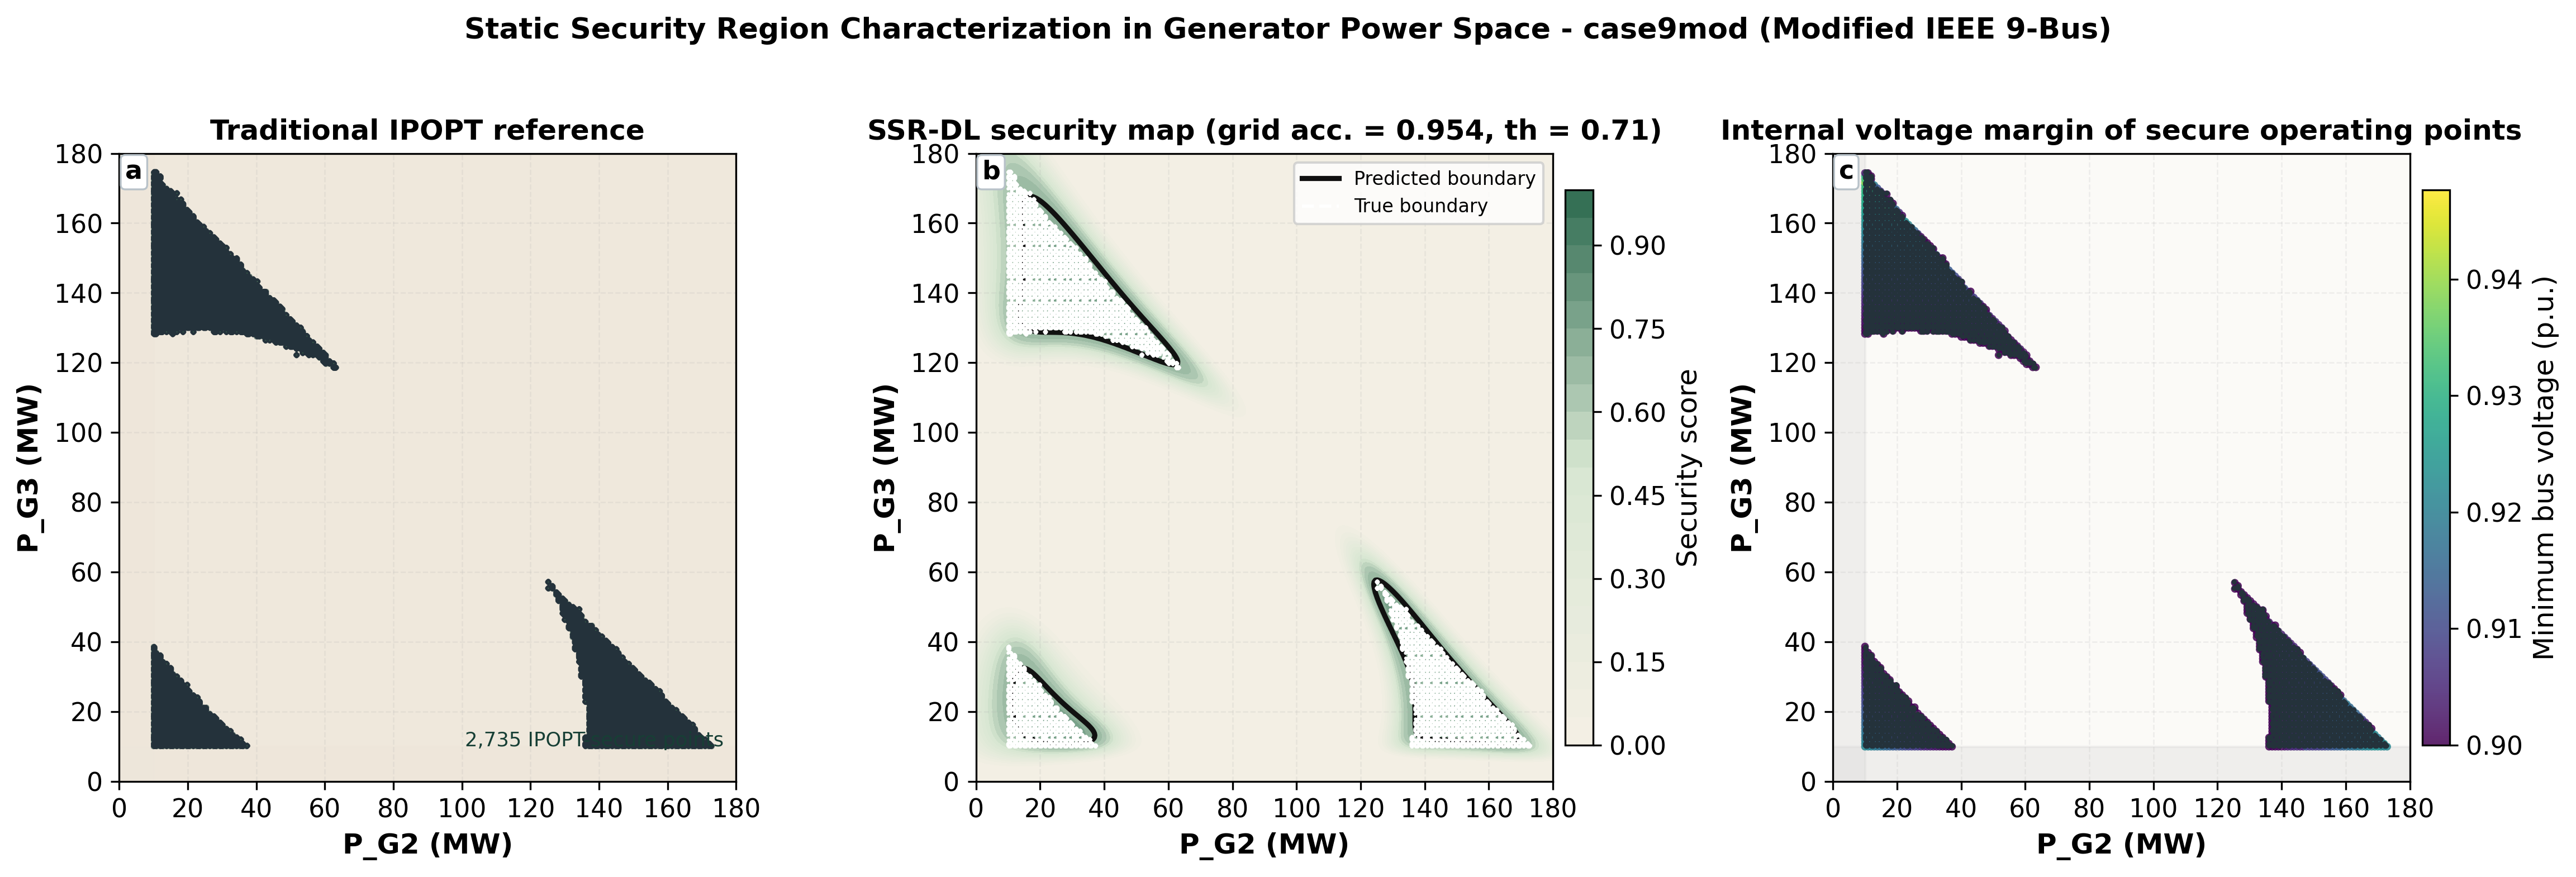
\includegraphics[width=\linewidth]{../figures/case9mod_security_region.png}
  \caption{case9mod security region projected onto the $(P_{L1}, P_{L2})$ plane.
    \textit{Left}: Ground truth. \textit{Center}: SSR-DL prediction.
    \textit{Right}: Error map (misclassified regions in dark red). Grid
    accuracy = 0.962.}
  \label{fig:case9mod_ssr}
\end{figure}

\begin{figure}[t]
  \centering
  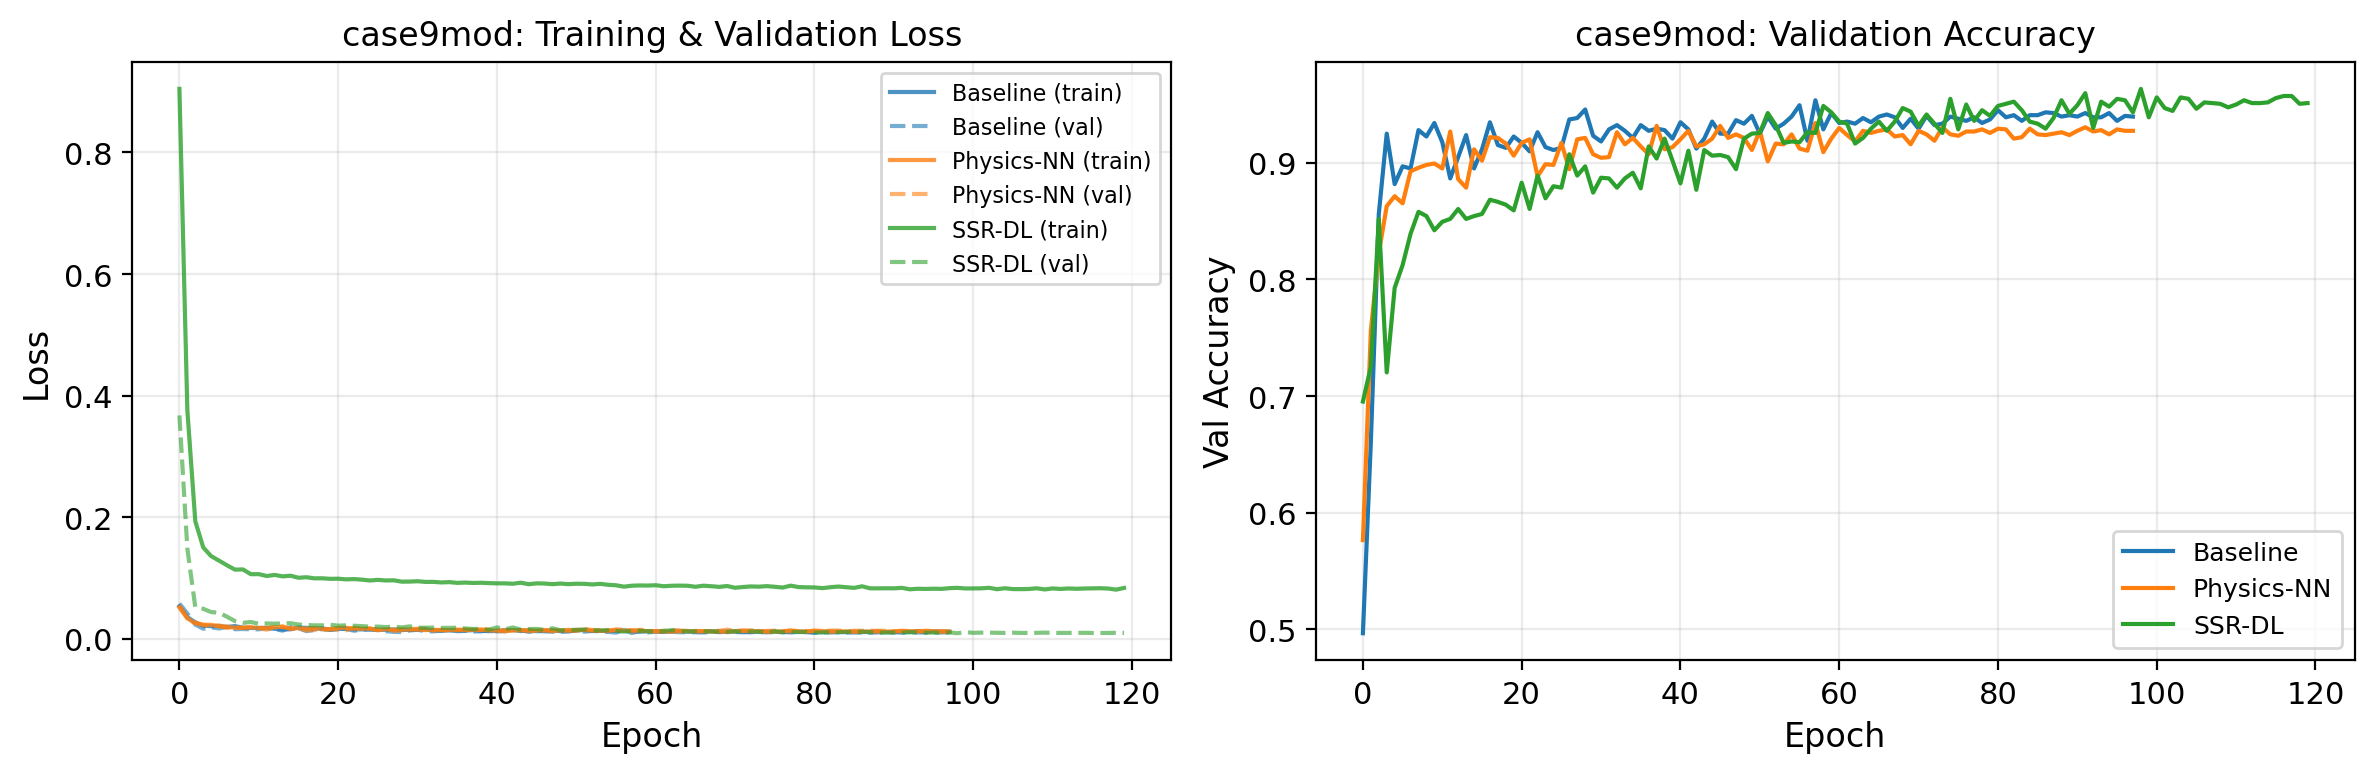
\includegraphics[width=\linewidth]{../figures/case9mod_training.png}
  \caption{Training dynamics for case9mod. SSR-DL achieves higher validation
    F1 than both baselines. The Lagrange multiplier $\lambda_V$ stabilizes
    around 0.90, indicating convergent dual variable evolution.}
  \label{fig:training}
\end{figure}

\begin{figure}[t]
  \centering
  \includegraphics[width=\linewidth]{../figures/WB2_roc_pr.png}
  \caption{ROC and PR curves for WB2. SSR-DL achieves AUC-ROC = AUC-PR = 1.000.}
  \label{fig:roc}
\end{figure}

% ─────────────────────────────────────────────────────────────────────────────
\bibliographystyle{IEEEtran}
\bibliography{references}
% ─────────────────────────────────────────────────────────────────────────────

\end{document}
